\documentclass{ximera}

\title{The Shell Method}
\author{Pat Smith}

\begin{document}
\begin{abstract}
We practice setting up setting up volume calculations using the shell method.
\end{abstract}
\maketitle

\begin{example}
The region defined by the inequalities $-\sqrt{1-x^2} \leq y \leq \sqrt{1-x^2}$ and $x \geq 0$ (shown below) is revolved around the $y$-ais. Compute the volume using the shell method.
\begin{center}
\begin{image}
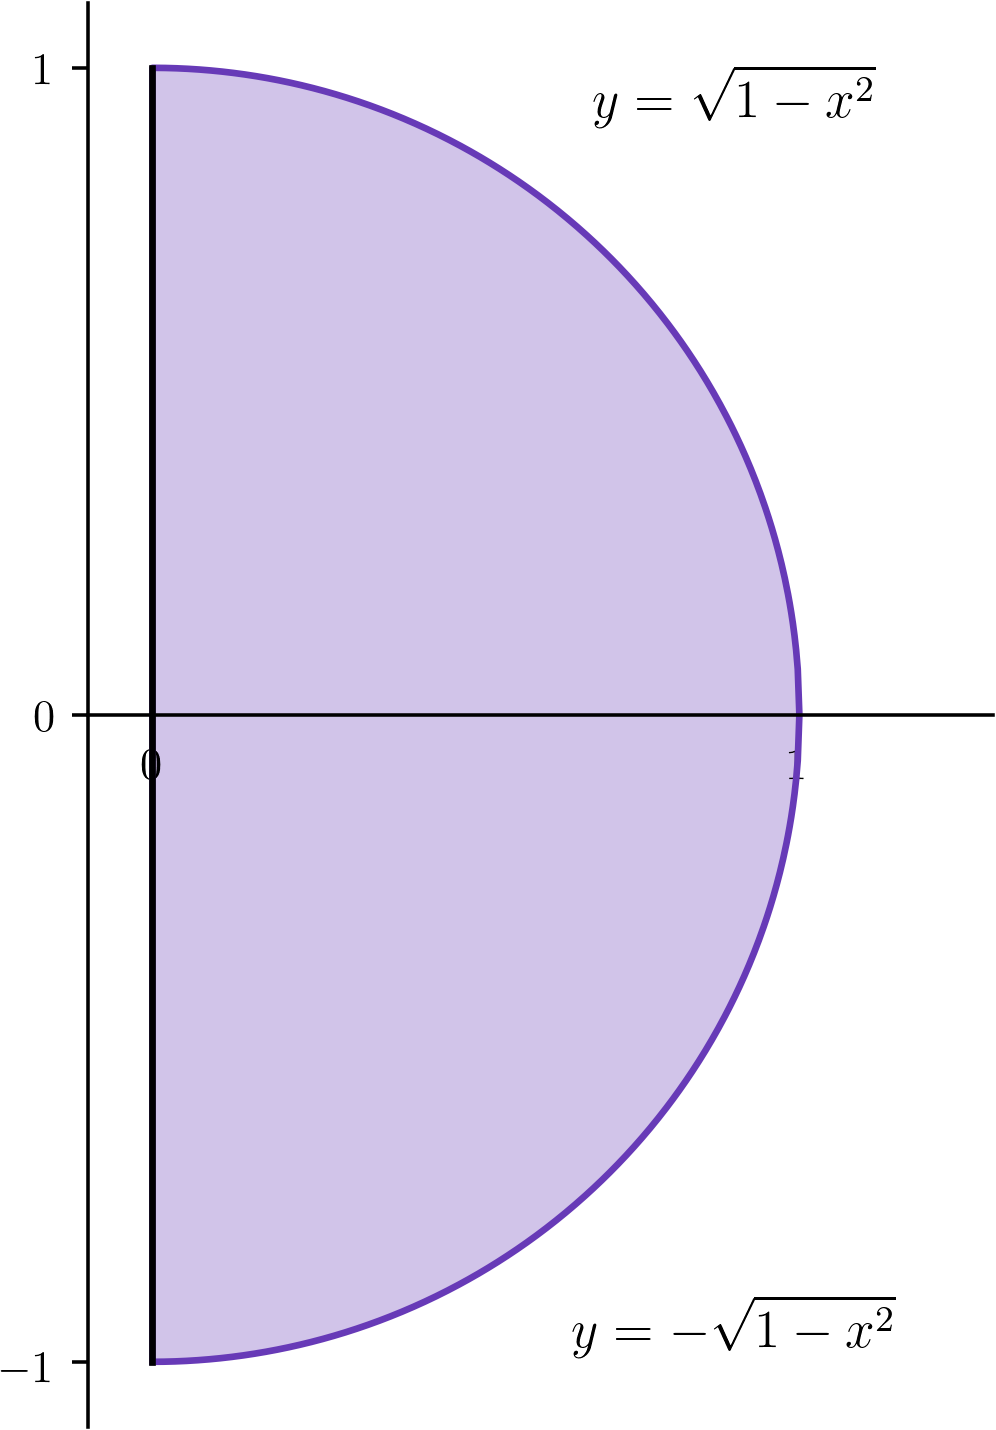
\includegraphics{shell/shell01.png}
\end{image}
\end{center}
\begin{itemize}
\item When the slicing variable is $x$, the radius of a shell is the \wordChoice{\choice[correct]{horizontal}\choice{vertical}} distance from an $x$-slice to the axis $x = 0$. Thus
\[ r(x) = \answer{x} - \answer{0}. \]
\item The height of an $x$-slice is equal to
\begin{multipleChoice}
\choice{$h(x) = \sqrt{1-x^2}$}
\choice{$h(x) = - \sqrt{1-x^2}$}
\choice[correct]{$h(x) = \sqrt{1-x^2} - \left( - \sqrt{1-x^2} \right) = 2 \sqrt{1-x^2}$}
\end{multipleChoice}
\item The volume is equal to the integral of $2 \pi r h$, so 
\[ V = \int_{\answer{0}}^{\answer{1}} \answer{4 \pi x \sqrt{1-x^2}} dx = \answer{\frac{4\pi}{3}}. \]
(Note: to compute the integral, we can make the substitution $u = 1-x^2$.)
\end{itemize}
\end{example}

\begin{example}
The region between the curves $x = \sqrt{y}$ and $x = y + \sqrt{y}$ from $y=0$ to $y=1$ is revolved around the axis $y=1$. Compute the volume of the resulting solid.
\begin{center}
\begin{image}
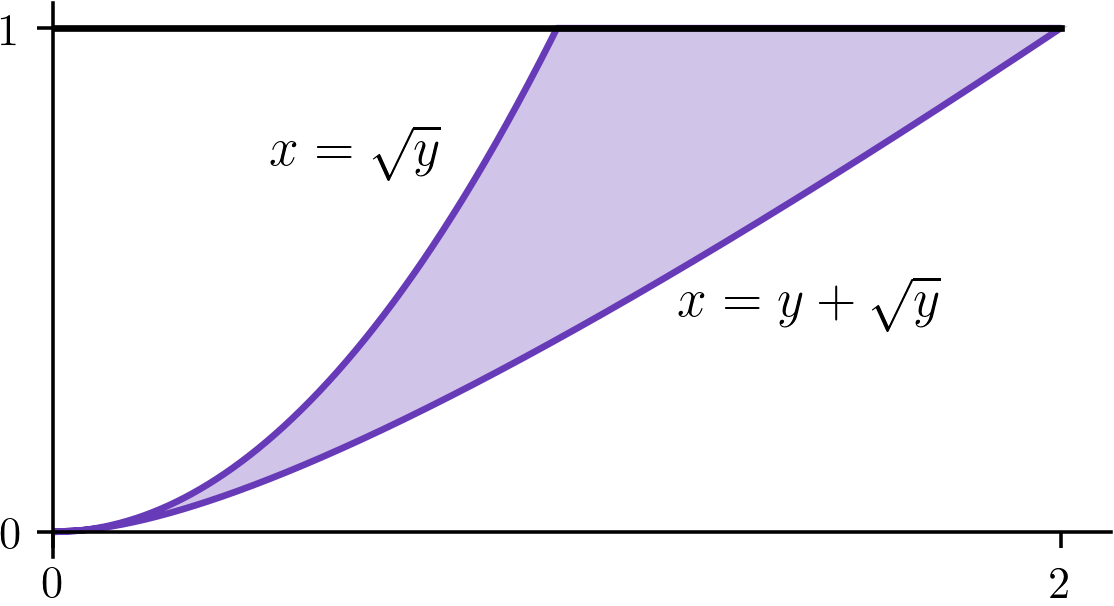
\includegraphics{shell/shell02.png}
\end{image}
\end{center}
\begin{itemize}
\item When the slicing variable is $y$, the radius of a shell is the \wordChoice{\choice{horizontal}\choice[correct]{vertical}} distance from a $y$-slice to the axis $y = 1$. Thus
\[ r(y) = \answer{1} - \answer{y}. \]
\item The ``height'' of a $y$-slice is equal to
\begin{multipleChoice}
\choice{$h(y) = \sqrt{y}$}
\choice{$h(y) = \sqrt{y} - (y + \sqrt{y}) = -y$}
\choice[correct]{$h(y) = (y + \sqrt{y}) - \sqrt{y} = y$}
\end{multipleChoice}
\item The volume is equal to the integral of $2 \pi r h$, so 
\[ V = \int_{\answer{0}}^{\answer{1}} \answer{2 \pi y(1-y)} dy = \answer{\frac{\pi}{3}}. \]
\end{itemize}
\end{example}



\end{document}
